% Options for packages loaded elsewhere
\PassOptionsToPackage{unicode}{hyperref}
\PassOptionsToPackage{hyphens}{url}
\PassOptionsToPackage{dvipsnames,svgnames*,x11names*}{xcolor}
%
\documentclass[
  10pt,
]{article}
\usepackage{lmodern}
\usepackage{amssymb,amsmath}
\usepackage{ifxetex,ifluatex}
\ifnum 0\ifxetex 1\fi\ifluatex 1\fi=0 % if pdftex
  \usepackage[T1]{fontenc}
  \usepackage[utf8]{inputenc}
  \usepackage{textcomp} % provide euro and other symbols
\else % if luatex or xetex
  \usepackage{unicode-math}
  \defaultfontfeatures{Scale=MatchLowercase}
  \defaultfontfeatures[\rmfamily]{Ligatures=TeX,Scale=1}
\fi
% Use upquote if available, for straight quotes in verbatim environments
\IfFileExists{upquote.sty}{\usepackage{upquote}}{}
\IfFileExists{microtype.sty}{% use microtype if available
  \usepackage[]{microtype}
  \UseMicrotypeSet[protrusion]{basicmath} % disable protrusion for tt fonts
}{}
\makeatletter
\@ifundefined{KOMAClassName}{% if non-KOMA class
  \IfFileExists{parskip.sty}{%
    \usepackage{parskip}
  }{% else
    \setlength{\parindent}{0pt}
    \setlength{\parskip}{6pt plus 2pt minus 1pt}}
}{% if KOMA class
  \KOMAoptions{parskip=half}}
\makeatother
\usepackage{xcolor}
\IfFileExists{xurl.sty}{\usepackage{xurl}}{} % add URL line breaks if available
\IfFileExists{bookmark.sty}{\usepackage{bookmark}}{\usepackage{hyperref}}
\hypersetup{
  colorlinks=true,
  linkcolor=Maroon,
  filecolor=Maroon,
  citecolor=Blue,
  urlcolor=Blue,
  pdfcreator={LaTeX via pandoc}}
\urlstyle{same} % disable monospaced font for URLs
\usepackage[margin=2.2cm]{geometry}
\usepackage{longtable,booktabs}
% Correct order of tables after \paragraph or \subparagraph
\usepackage{etoolbox}
\makeatletter
\patchcmd\longtable{\par}{\if@noskipsec\mbox{}\fi\par}{}{}
\makeatother
% Allow footnotes in longtable head/foot
\IfFileExists{footnotehyper.sty}{\usepackage{footnotehyper}}{\usepackage{footnote}}
\makesavenoteenv{longtable}
\usepackage{graphicx}
\makeatletter
\def\maxwidth{\ifdim\Gin@nat@width>\linewidth\linewidth\else\Gin@nat@width\fi}
\def\maxheight{\ifdim\Gin@nat@height>\textheight\textheight\else\Gin@nat@height\fi}
\makeatother
% Scale images if necessary, so that they will not overflow the page
% margins by default, and it is still possible to overwrite the defaults
% using explicit options in \includegraphics[width, height, ...]{}
\setkeys{Gin}{width=\maxwidth,height=\maxheight,keepaspectratio}
% Set default figure placement to htbp
\makeatletter
\def\fps@figure{htbp}
\makeatother
\setlength{\emergencystretch}{3em} % prevent overfull lines
\providecommand{\tightlist}{%
  \setlength{\itemsep}{0pt}\setlength{\parskip}{0pt}}
\setcounter{secnumdepth}{-\maxdimen} % remove section numbering
\usepackage{amssymb}
\usepackage{newunicodechar}
\newunicodechar{≥}{\ensuremath{\geq}}
\newunicodechar{≤}{\ensuremath{\leq}}
\newunicodechar{−}{\ensuremath{-}}
\newunicodechar{×}{\ensuremath{\times}}
\newunicodechar{▲}{\ensuremath{\blacktriangle}}
\newunicodechar{△}{\ensuremath{\vartriangle}}
\newunicodechar{◆}{\ensuremath{\blacklozenge}}
\newunicodechar{●}{\ensuremath{\bullet}}
\newunicodechar{▶}{\ensuremath{\blacktriangleright}}
\newunicodechar{❚}{\textbf{|}}
\setkeys{Gin}{width=\linewidth,height=0.6\textheight,keepaspectratio}
\usepackage{parskip}

\title{How to use the Nepal flood forecast}
\usepackage{etoolbox}
\makeatletter
\providecommand{\subtitle}[1]{% add subtitle to \maketitle
  \apptocmd{\@title}{\par {\large #1 \par}}{}{}
}
\makeatother
\subtitle{A guide for readers}
\author{}
\date{}

\begin{document}
\maketitle

{
\hypersetup{linkcolor=}
\setcounter{tocdepth}{3}
\tableofcontents
}
\hypertarget{how-to-use-the-nepal-flood-forecast-a-guide-for-readers}{%
\section{How to use the Nepal flood forecast: a guide for
readers}\label{how-to-use-the-nepal-flood-forecast-a-guide-for-readers}}

\textbf{Live page:
https://sauravbhattarai19.github.io/Nepal\_Empirical\_Flood\_Forecast/}

This guide explains every part of the page: what each number means,
where it comes from, how the page boils three weather models and nine
formulas down to one colour per river, and what you can (and cannot)
learn from it. No hydrology background is needed; the
\href{methods.md}{methods} give the formulas for those who want them.

\begin{quote}
\textbf{An experimental research forecast, not a flood warning.} The
numbers come from weather-model rain and Nepal's empirical formulas and
have not been checked against measured floods at these rivers. For
official forecasts and warnings, follow the Department of Hydrology and
Meteorology (\href{https://www.hydrology.gov.np}{hydrology.gov.np}) and
your local authorities.
\end{quote}

\begin{quote}
\textbf{Two kinds of screenshots.} Pictures marked \emph{real} show the
actual forecast of 1 November 2026, a dry day with no floods. To show
what a flood looks like, the other pictures use a \textbf{made-up storm}
fed through the same code; they carry a black-and-yellow label
\emph{``MADE-UP STORM · illustration, not a forecast''}. None of their
numbers is a forecast for any river.
\end{quote}

\hypertarget{the-page-at-a-glance}{%
\subsection{1. The page at a glance}\label{the-page-at-a-glance}}

\emph{Real, 1 November 2026, 01:46 Nepal time.}

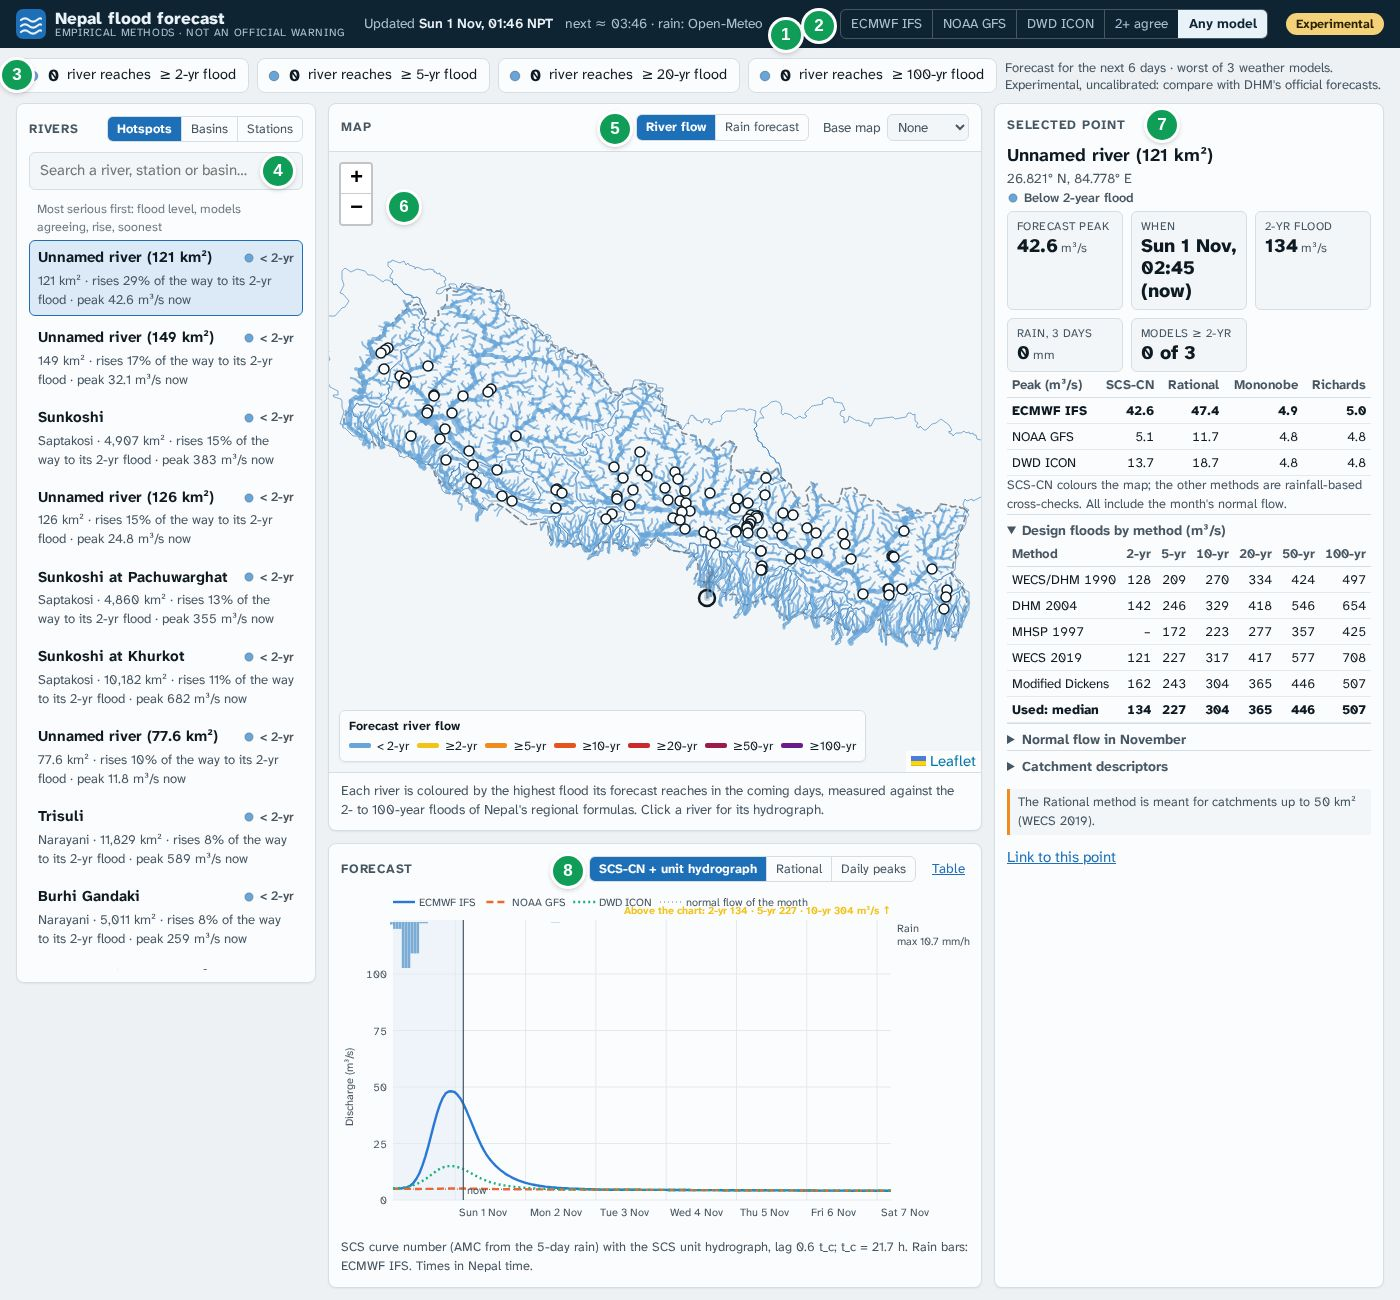
\includegraphics{img/guide/01-overview.jpg}

\begin{longtable}[]{@{}lll@{}}
\toprule
\begin{minipage}[b]{0.30\columnwidth}\raggedright
\strut
\end{minipage} & \begin{minipage}[b]{0.30\columnwidth}\raggedright
Part\strut
\end{minipage} & \begin{minipage}[b]{0.30\columnwidth}\raggedright
What it is for\strut
\end{minipage}\tabularnewline
\midrule
\endhead
\begin{minipage}[t]{0.30\columnwidth}\raggedright
\textbf{1}\strut
\end{minipage} & \begin{minipage}[t]{0.30\columnwidth}\raggedright
Update line\strut
\end{minipage} & \begin{minipage}[t]{0.30\columnwidth}\raggedright
When this forecast was made, when the next one is due, and where the
rain came from (normally \emph{Open-Meteo})\strut
\end{minipage}\tabularnewline
\begin{minipage}[t]{0.30\columnwidth}\raggedright
\textbf{2}\strut
\end{minipage} & \begin{minipage}[t]{0.30\columnwidth}\raggedright
View buttons\strut
\end{minipage} & \begin{minipage}[t]{0.30\columnwidth}\raggedright
Which weather model the whole page shows: one of the three, \textbf{2+
agree} or \textbf{Any model}
(\protect\hyperlink{4-the-top-bar-update-time-and-the-five-views}{section
4})\strut
\end{minipage}\tabularnewline
\begin{minipage}[t]{0.30\columnwidth}\raggedright
\textbf{3}\strut
\end{minipage} & \begin{minipage}[t]{0.30\columnwidth}\raggedright
Summary chips\strut
\end{minipage} & \begin{minipage}[t]{0.30\columnwidth}\raggedright
How many river reaches reach the 2-, 5-, 20- and 100-year flood in the
chosen view\strut
\end{minipage}\tabularnewline
\begin{minipage}[t]{0.30\columnwidth}\raggedright
\textbf{4}\strut
\end{minipage} & \begin{minipage}[t]{0.30\columnwidth}\raggedright
Rivers list\strut
\end{minipage} & \begin{minipage}[t]{0.30\columnwidth}\raggedright
The most serious rivers first, or the big river systems, or the DHM
stations, or a search
(\protect\hyperlink{7-the-rivers-list-hotspots-basins-stations-search}{section
7})\strut
\end{minipage}\tabularnewline
\begin{minipage}[t]{0.30\columnwidth}\raggedright
\textbf{5}\strut
\end{minipage} & \begin{minipage}[t]{0.30\columnwidth}\raggedright
Map layer\strut
\end{minipage} & \begin{minipage}[t]{0.30\columnwidth}\raggedright
\textbf{River flow} (rivers coloured by flood level) or \textbf{Rain
forecast} (rain on a grid), and the base map\strut
\end{minipage}\tabularnewline
\begin{minipage}[t]{0.30\columnwidth}\raggedright
\textbf{6}\strut
\end{minipage} & \begin{minipage}[t]{0.30\columnwidth}\raggedright
Map\strut
\end{minipage} & \begin{minipage}[t]{0.30\columnwidth}\raggedright
Every river of Nepal draining at least 20 km² (about 4,200 reaches) and
the 112 DHM stations (white circles)\strut
\end{minipage}\tabularnewline
\begin{minipage}[t]{0.30\columnwidth}\raggedright
\textbf{7}\strut
\end{minipage} & \begin{minipage}[t]{0.30\columnwidth}\raggedright
Selected point\strut
\end{minipage} & \begin{minipage}[t]{0.30\columnwidth}\raggedright
Everything about the river you clicked: peak, timing, flood levels,
every method's numbers
(\protect\hyperlink{8-selected-point-everything-shown-when-you-click-a-river}{section
8})\strut
\end{minipage}\tabularnewline
\begin{minipage}[t]{0.30\columnwidth}\raggedright
\textbf{8}\strut
\end{minipage} & \begin{minipage}[t]{0.30\columnwidth}\raggedright
Forecast chart\strut
\end{minipage} & \begin{minipage}[t]{0.30\columnwidth}\raggedright
The forecast flow of that river hour by hour, with its flood levels
(\protect\hyperlink{10-the-forecast-chart-hydrograph}{section 10})\strut
\end{minipage}\tabularnewline
\bottomrule
\end{longtable}

When the page opens, it selects the first river of the Hotspots list for
you.

\hypertarget{a-five-minute-routine}{%
\subsection{2. A five-minute routine}\label{a-five-minute-routine}}

\begin{enumerate}
\def\labelenumi{\arabic{enumi}.}
\tightlist
\item
  \textbf{Check the update line (1).} It should say \emph{Updated}
  within the last 2 to 3 hours. A red \textbf{Late} label means the last
  update is more than 6 hours old. If the line names a backup source
  instead of Open-Meteo, only one weather model is available.
\item
  \textbf{Read the chips (3).} All zeros (as in the real screenshot)
  means no river reaches even its 2-year flood in the coming days, in
  the chosen view.
\item
  \textbf{Switch between ``Any model'' and ``2+ agree'' (2).} \emph{Any
  model} is the worst case: the page opens on it. \emph{2+ agree} shows
  only what at least two of the three models say. A river coloured in
  both is a stronger signal than a river coloured in \emph{Any model}
  only.
\item
  \textbf{Open the Hotspots list (4)} and click the first rivers. For
  each, look at \textbf{when} the peak comes, \textbf{how many models}
  reach that level, and the \textbf{chart}: do the three model lines
  agree, and is the rain that causes the peak still days away?
\item
  \textbf{Open the rain map (5)} and press ▶ to see where and when the
  rain falls.
\item
  \textbf{Compare with official sources} before acting on anything.
\end{enumerate}

\hypertarget{what-a-2-year-flood-means}{%
\subsection{3. What a ``2-year flood''
means}\label{what-a-2-year-flood-means}}

Every river point on the page has six \textbf{flood levels}, in m³/s
(cubic metres of water per second): the \textbf{2-, 5-, 10-, 20-, 50-
and 100-year floods}.

\begin{itemize}
\tightlist
\item
  A \textbf{2-year flood} is a flow that the river reaches or exceeds,
  on average, in one year out of two (a 50\% chance in any year). It is
  a high-water mark the river reaches often: the banks are full and low
  fields may get wet, but it is not a disaster.
\item
  A \textbf{5-year flood} has a 20\% chance in any year, a
  \textbf{20-year flood} 5\%, and a \textbf{100-year flood} 1\%. These
  are rare, damaging floods.
\item
  It is a probability, not a timetable. Two ``100-year floods'' can come
  in consecutive years.
\end{itemize}

These levels are not measured at each river: they come from
\textbf{Nepal's regional flood formulas} (WECS/DHM 1990, DHM 2004, MHSP
1997, WECS 2019 and Modified Dickens), which estimate floods from the
catchment area and elevation. The page uses the \textbf{median} of the
five formulas and shows all of them for every point
(\protect\hyperlink{design-floods-by-method}{section 8}).

The page always shows a level with a \textbf{colour, a shape and words},
so it can be read without colour vision too:

\begin{longtable}[]{@{}lll@{}}
\toprule
Shape & Colour & Words\tabularnewline
\midrule
\endhead
● circle & blue & \emph{Below 2-year flood} / \emph{\textless{}
2-yr}\tabularnewline
▲ triangle & yellow, orange & \emph{≥ 2-year flood}, \emph{≥ 5-year
flood}\tabularnewline
◆ diamond & red-orange, red & \emph{≥ 10-year flood}, \emph{≥ 20-year
flood}\tabularnewline
octagon & dark red, purple & \emph{≥ 50-year flood}, \emph{≥ 100-year
flood}\tabularnewline
\bottomrule
\end{longtable}

\hypertarget{the-top-bar-update-time-and-the-five-views}{%
\subsection{4. The top bar: update time and the five
views}\label{the-top-bar-update-time-and-the-five-views}}

The forecast is remade \textbf{every 2 hours} on GitHub's servers. Each
update downloads the latest hourly rain forecasts of three global
weather models from Open-Meteo:

\begin{itemize}
\tightlist
\item
  \textbf{ECMWF IFS}, the European Centre's model
\item
  \textbf{NOAA GFS}, the US model
\item
  \textbf{DWD ICON}, the German model
\end{itemize}

They often disagree, especially on \emph{where} heavy rain falls, so the
page lets you choose how to look at them:

\begin{longtable}[]{@{}lll@{}}
\toprule
\begin{minipage}[b]{0.30\columnwidth}\raggedright
Button\strut
\end{minipage} & \begin{minipage}[b]{0.30\columnwidth}\raggedright
What the page shows\strut
\end{minipage} & \begin{minipage}[b]{0.30\columnwidth}\raggedright
When to use it\strut
\end{minipage}\tabularnewline
\midrule
\endhead
\begin{minipage}[t]{0.30\columnwidth}\raggedright
\textbf{ECMWF IFS}, \textbf{NOAA GFS}, \textbf{DWD ICON}\strut
\end{minipage} & \begin{minipage}[t]{0.30\columnwidth}\raggedright
That model alone\strut
\end{minipage} & \begin{minipage}[t]{0.30\columnwidth}\raggedright
To see one model's story; its chart line is drawn bold, the others
faint\strut
\end{minipage}\tabularnewline
\begin{minipage}[t]{0.30\columnwidth}\raggedright
\textbf{2+ agree}\strut
\end{minipage} & \begin{minipage}[t]{0.30\columnwidth}\raggedright
For each river, the highest level that \textbf{at least two} models
reach\strut
\end{minipage} & \begin{minipage}[t]{0.30\columnwidth}\raggedright
The more confident picture: fewer false alarms\strut
\end{minipage}\tabularnewline
\begin{minipage}[t]{0.30\columnwidth}\raggedright
\textbf{Any model} \emph{(default)}\strut
\end{minipage} & \begin{minipage}[t]{0.30\columnwidth}\raggedright
For each river, the highest level that \textbf{any} model reaches\strut
\end{minipage} & \begin{minipage}[t]{0.30\columnwidth}\raggedright
The worst case: nothing is missed, but more false alarms\strut
\end{minipage}\tabularnewline
\bottomrule
\end{longtable}

The made-up storm below shows the five views of the same forecast side
by side. In it, ECMWF puts its heaviest rain around Pokhara, GFS further
east and ICON is weaker. \textbf{Any model} is the union of all three
(983 reaches ≥ 2-yr), \textbf{2+ agree} keeps only where two models
overlap (355 reaches):

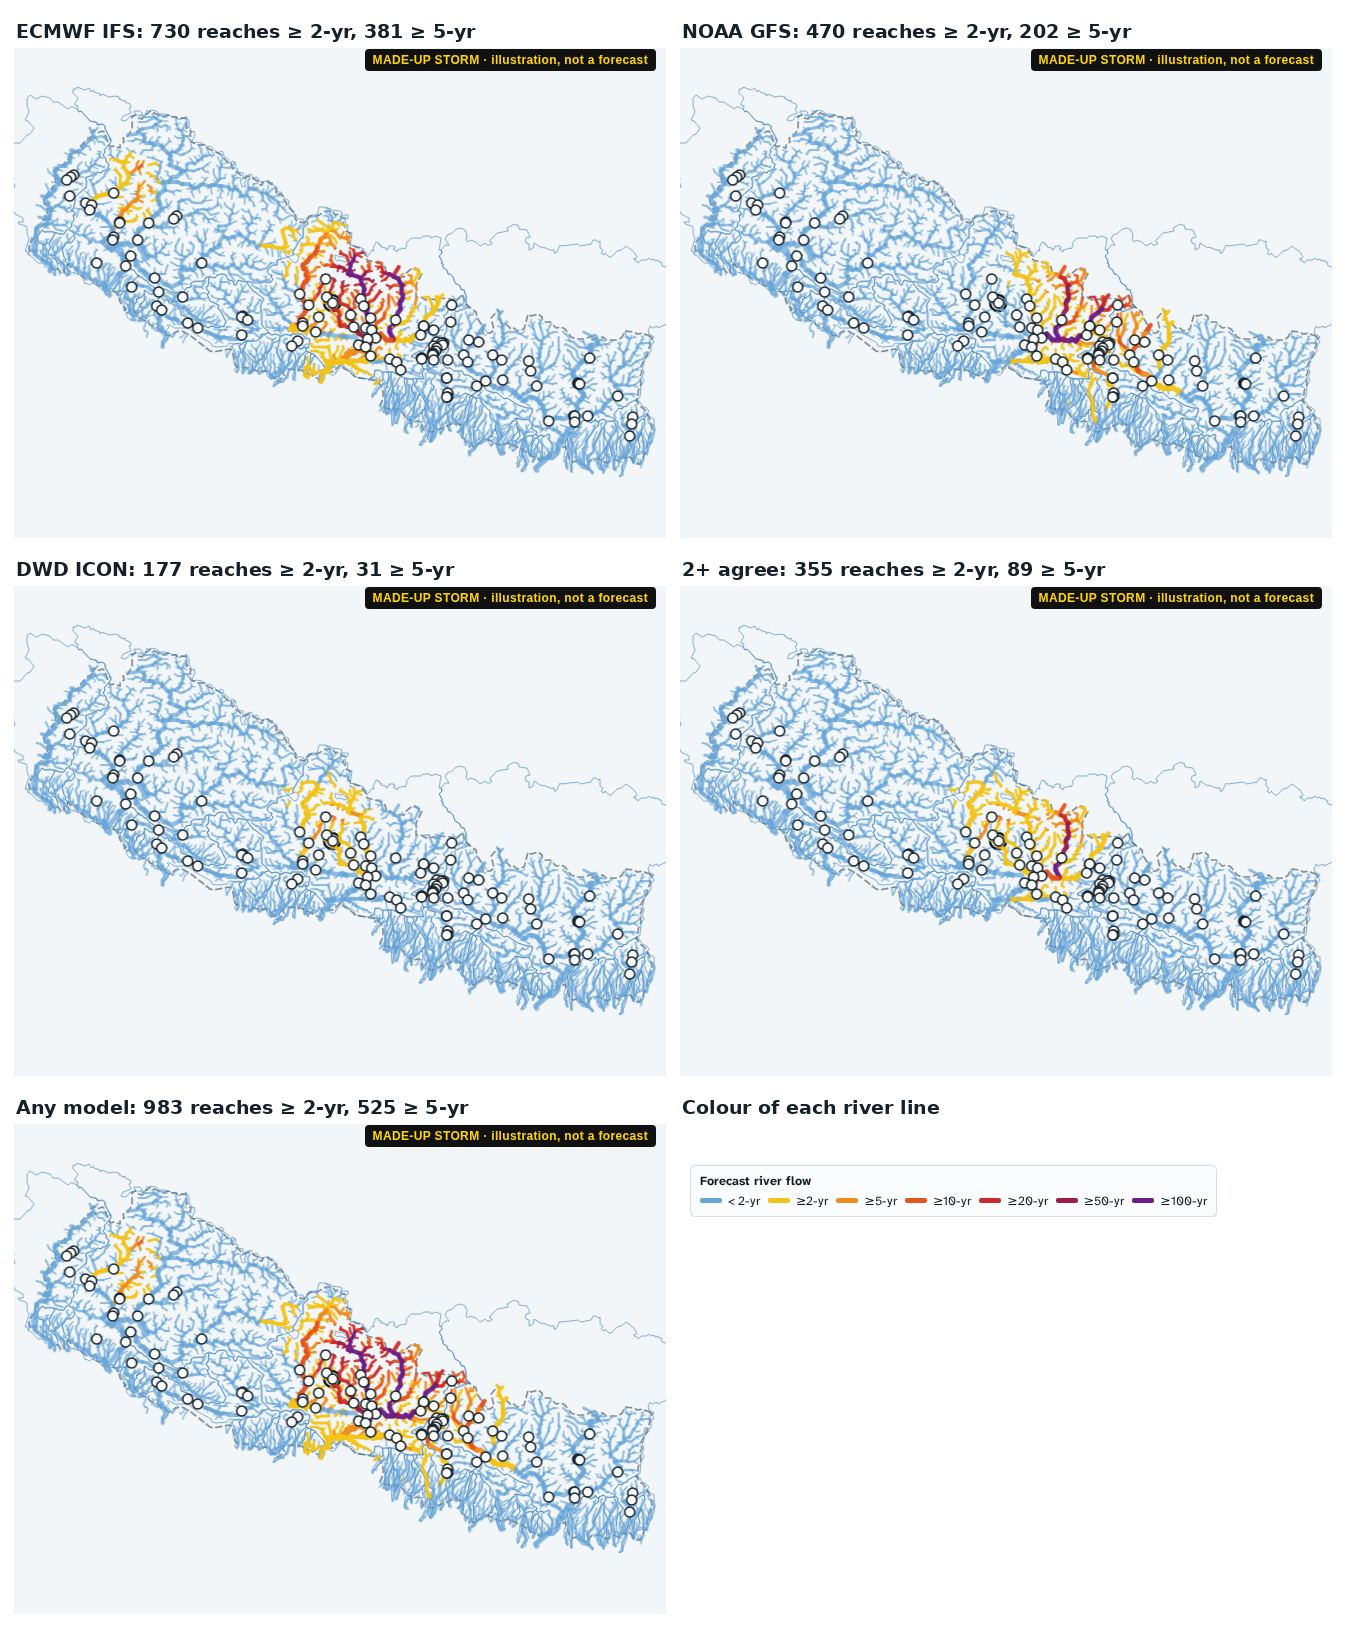
\includegraphics{img/guide/03-five-views.jpg}

The line under the chips says which view you are in (``worst of 3
weather models'', ``what at least 2 of 3 weather models agree on'', or
the model's name) and how many days ahead the forecast goes (6 to 7).

\hypertarget{the-map-river-flow}{%
\subsection{5. The map: river flow}\label{the-map-river-flow}}

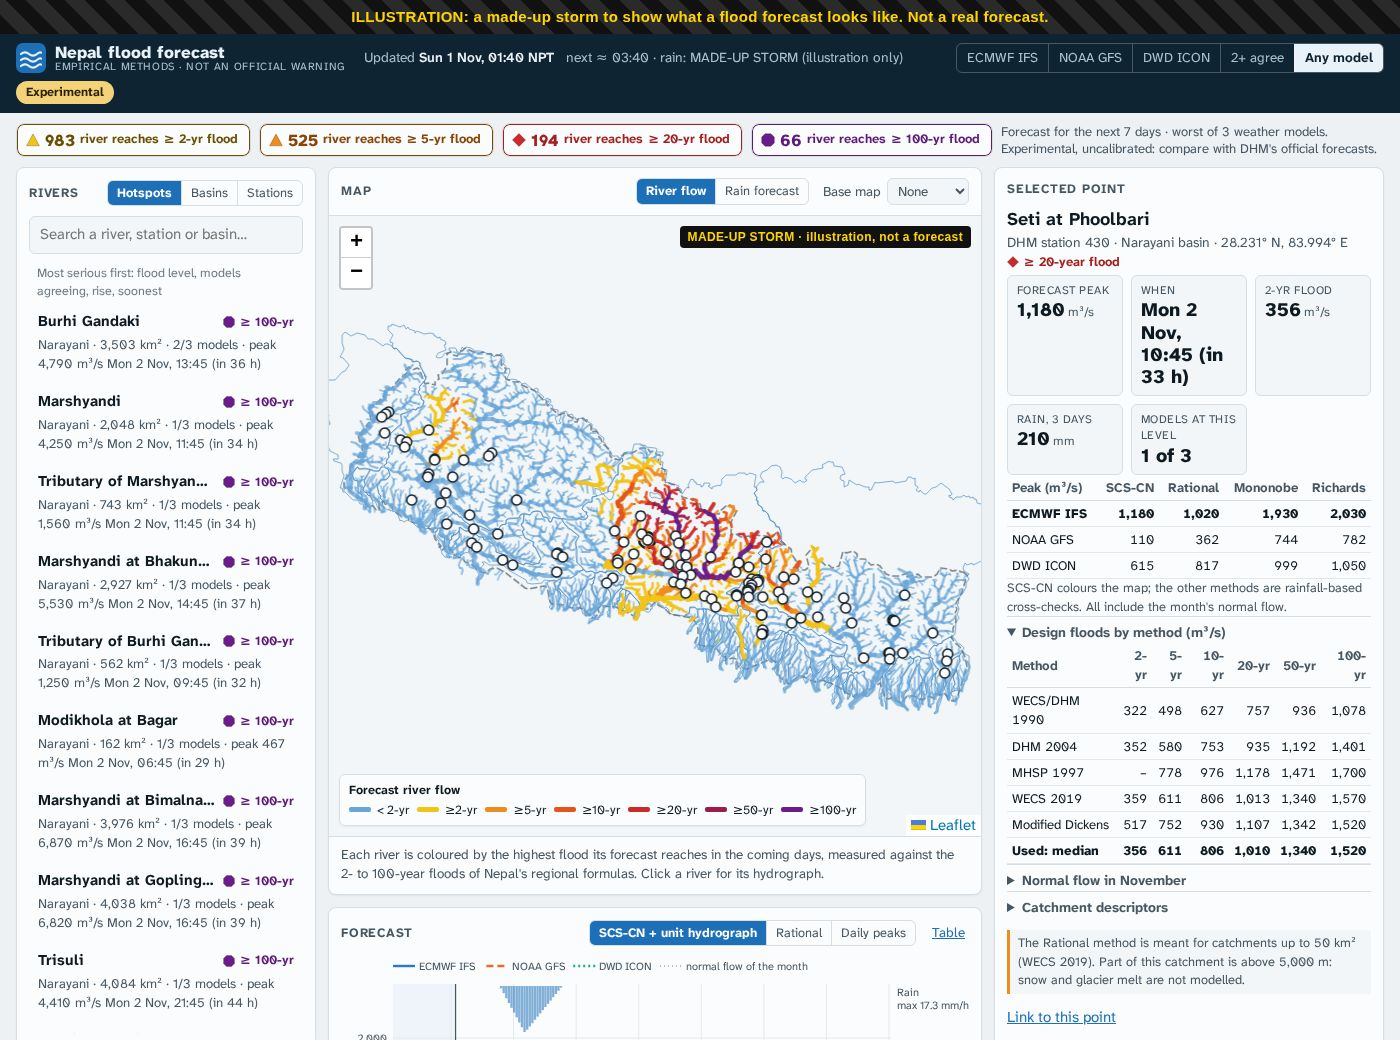
\includegraphics{img/guide/02-storm-overview.jpg}

\begin{itemize}
\tightlist
\item
  \textbf{Colour}: the highest flood level the river's forecast reaches
  \textbf{at any time from now to the end of the forecast}, in the
  chosen view. Blue = stays below its 2-year flood. The colour does not
  say \emph{when}: click the river for that.
\item
  \textbf{Line width}: bigger rivers (larger drainage area) are drawn
  thicker.
\item
  \textbf{White circles}: the 112 DHM hydrometric stations.
  \textbf{Dashed grey line}: Nepal's border. \textbf{Thin blue
  outlines}: the 75 river systems that leave Nepal.
\item
  \textbf{Hover} over a river for its name, drainage area, forecast
  peak, level and 2-year flood.
\item
  \textbf{Click} a river or station to select it. A ring marks the point
  and a faint grey halo marks every river upstream of it, that is, the
  catchment whose rain feeds it.
\end{itemize}

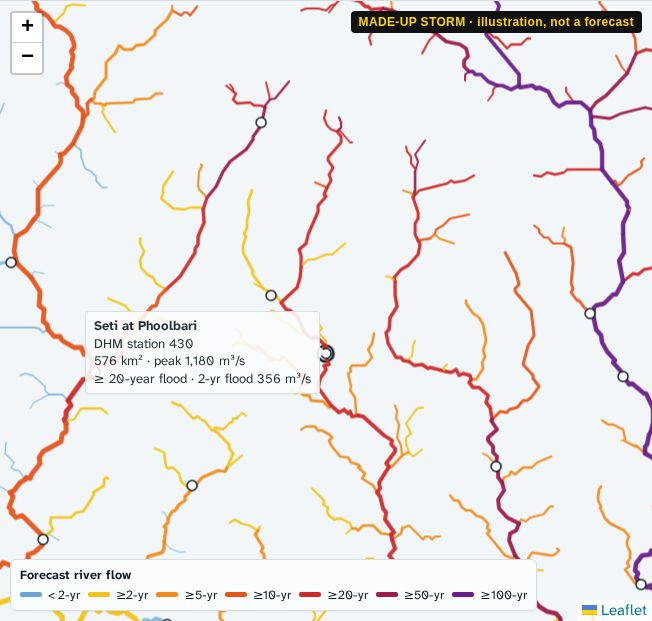
\includegraphics{img/guide/04-hover-and-catchment.jpg}

The tooltip above reads: \emph{Seti at Phoolbari, DHM station 430, 576
km², peak 1,180 m³/s, ≥ 20-year flood, 2-year flood 356 m³/s}. In words:
in the worst model, this river is forecast to carry more than three
times its 2-year flood.

\textbf{Base map.} The map opens with \textbf{None}, plain rivers on a
light background, which is the clearest for reading flood colours.
Choose \textbf{Terrain}, \textbf{Streets} or \textbf{Satellite} to see
villages, roads and hills underneath; your browser remembers the choice.

\textbf{Zoom} with the + and − buttons, the mouse wheel or two fingers.
Even the smallest coloured line is a real river of at least 20 km².

\hypertarget{the-map-rain-forecast}{%
\subsection{6. The map: rain forecast}\label{the-map-rain-forecast}}

Press \textbf{Rain forecast} above the map. The rain is drawn as squares
of 0.25° (about 25 km): one square per point of the weather-model grid.

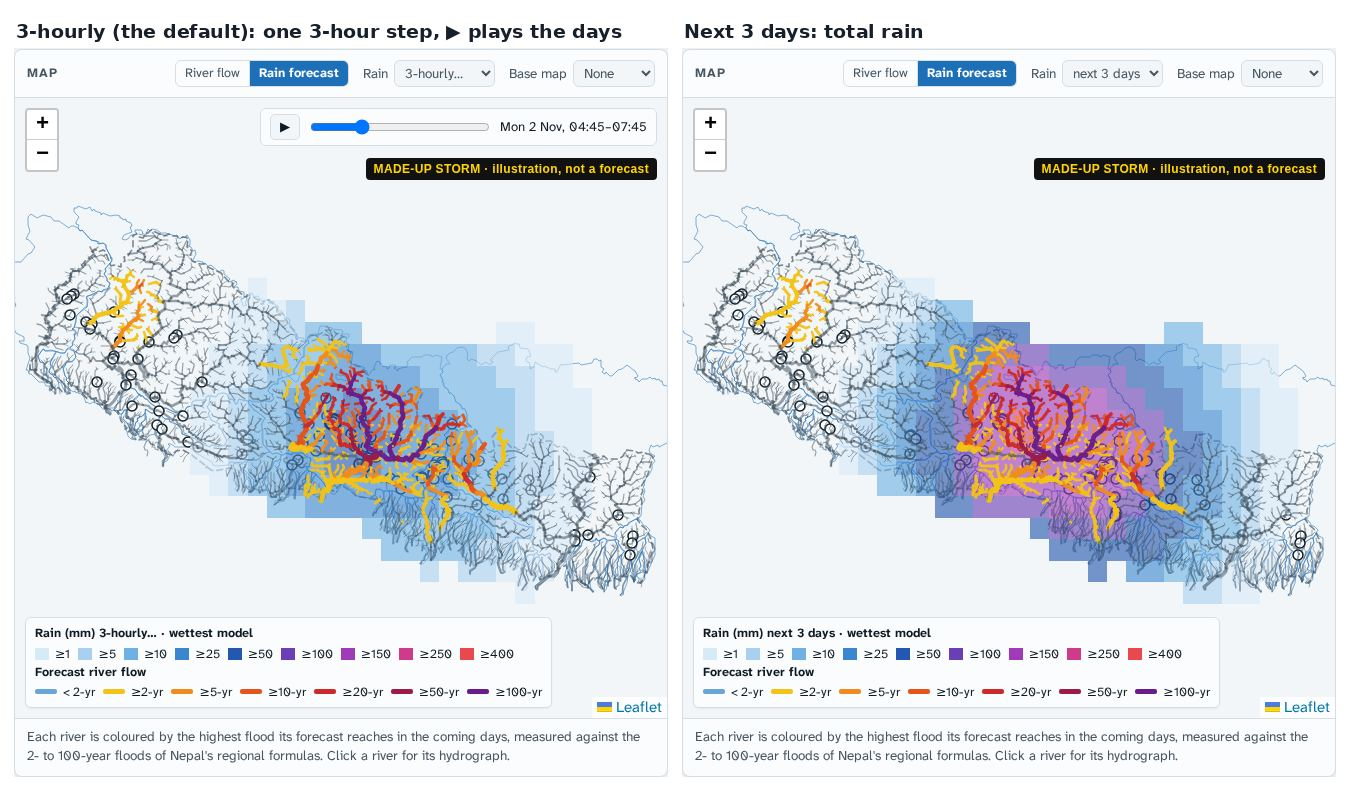
\includegraphics{img/guide/05-rain-map.jpg}

\begin{itemize}
\tightlist
\item
  The layer opens on \textbf{3-hourly}: the rain of one 3-hour window,
  starting with the current one. The time is shown next to the slider in
  the top-right corner. Press \textbf{▶} to play through the days (it
  loops), \textbf{❚❚} to pause, or drag the slider. The slider starts 24
  hours in the past, so you can also replay the rain that has already
  fallen.
\item
  The \textbf{Rain} menu also offers totals: \textbf{next 24 h},
  \textbf{next 3 days}, \textbf{next 7 days} and \textbf{past 24 h}.
\item
  In \textbf{Any model} and \textbf{2+ agree} the squares show the
  \textbf{wettest model} in each square; pick a single model to see its
  own rain.
\item
  Rivers below their 2-year flood turn grey so the rain stands out;
  rivers at a flood level keep their colour, so you can see which rain
  is causing which flood.
\item
  Hover over a square for its exact amount in mm.
\end{itemize}

What to look for: rain over the \textbf{upper catchment} of a river
reaches the plains hours to days later. Heavy rain in the hills today
can mean a flood downstream tomorrow.

\hypertarget{the-rivers-list-hotspots-basins-stations-search}{%
\subsection{7. The Rivers list: Hotspots, Basins, Stations,
search}\label{the-rivers-list-hotspots-basins-stations-search}}

\hypertarget{hotspots}{%
\subsubsection{Hotspots}\label{hotspots}}

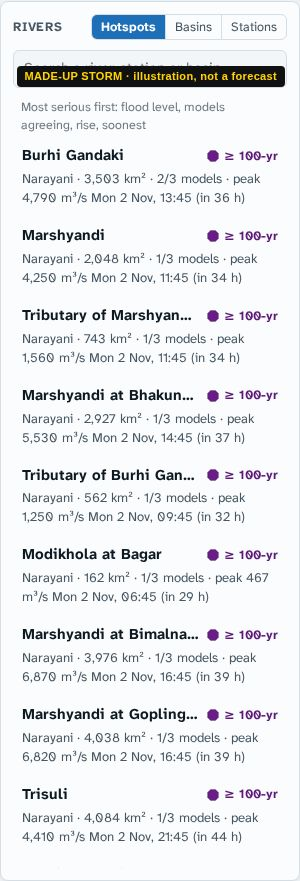
\includegraphics{img/guide/06-hotspots.jpg}

The most serious rivers come first, ranked by:

\begin{enumerate}
\def\labelenumi{\arabic{enumi}.}
\tightlist
\item
  the \textbf{flood level} reached (100-year before 50-year \ldots),
\item
  then \textbf{how many models} reach it,
\item
  then \textbf{how far the river rises} towards its 2-year flood,
\item
  then the \textbf{soonest} peak.
\end{enumerate}

Each river appears once (at its most serious point); stations and your
own points are listed separately. The list shows up to 60 lines and
stops early when the rest are quiet. On a dry day the caption says
\emph{``No river is forecast to rise noticeably''}.

How to read a line:

\begin{longtable}[]{@{}ll@{}}
\toprule
\begin{minipage}[b]{0.47\columnwidth}\raggedright
Example\strut
\end{minipage} & \begin{minipage}[b]{0.47\columnwidth}\raggedright
Meaning\strut
\end{minipage}\tabularnewline
\midrule
\endhead
\begin{minipage}[t]{0.47\columnwidth}\raggedright
\textbf{Burhi Gandaki} · ≥ 100-yrNarayani · 3,503 km² · 2/3 models ·
peak 4,790 m³/s Mon 2 Nov, 13:45 (in 36 h)\strut
\end{minipage} & \begin{minipage}[t]{0.47\columnwidth}\raggedright
Basin Narayani, drainage area 3,503 km². Two of the three models reach
the 100-year flood here. The highest flow, 4,790 m³/s, is forecast for
Monday 13:45, 36 hours from now\strut
\end{minipage}\tabularnewline
\begin{minipage}[t]{0.47\columnwidth}\raggedright
\textbf{Unnamed river (121 km²)} · \textless{} 2-yr121 km² · rises 29\%
of the way to its 2-yr flood · peak 42.6 m³/s now\strut
\end{minipage} & \begin{minipage}[t]{0.47\columnwidth}\raggedright
Below its 2-year flood. Its flow is 29\% of the way from its normal flow
(for the month) to its 2-year flood, and the highest value is
\emph{now}, so it is already falling (see
\protect\hyperlink{11-reading-a-quiet-day}{section 11})\strut
\end{minipage}\tabularnewline
\begin{minipage}[t]{0.47\columnwidth}\raggedright
\ldots{} · no rise forecast, 18.0 m³/s \emph{(example)}\strut
\end{minipage} & \begin{minipage}[t]{0.47\columnwidth}\raggedright
The forecast stays within about 5\% of the normal flow of the
month\strut
\end{minipage}\tabularnewline
\bottomrule
\end{longtable}

\hypertarget{basins}{%
\subsubsection{Basins}\label{basins}}

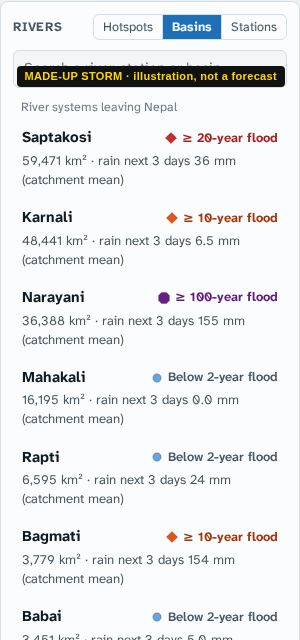
\includegraphics{img/guide/07-basins-list.jpg}

The 75 river systems that leave Nepal (Saptakosi, Karnali, Narayani
\ldots), largest first. The badge is the highest level reached anywhere
in that basin in the chosen view; the line gives the \textbf{mean rain
over the whole basin for the next 3 days} (the wettest model in the
combined views). Clicking a basin selects its outlet, where it leaves
Nepal.

\hypertarget{stations}{%
\subsubsection{Stations}\label{stations}}

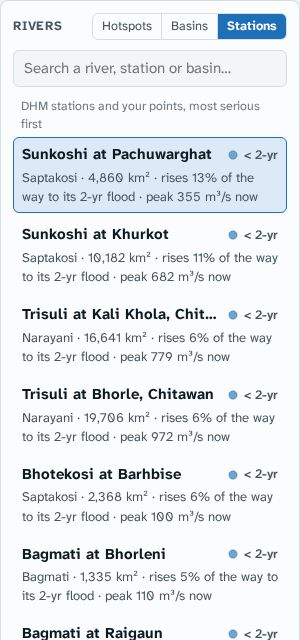
\includegraphics{img/guide/07-stations-list.jpg}

The 112 DHM hydrometric stations (and any points added by the operator),
ranked like the hotspots. Use it to check a forecast against the water
levels DHM publishes.

\hypertarget{search}{%
\subsubsection{Search}\label{search}}

Type part of a river, station or basin name, or a DHM station number
(e.g.~\emph{DHM 430}). Only named points appear in the results, largest
first.

\hypertarget{selected-point-everything-shown-when-you-click-a-river}{%
\subsection{8. Selected point: everything shown when you click a
river}\label{selected-point-everything-shown-when-you-click-a-river}}

\emph{Made-up storm, Any model.}

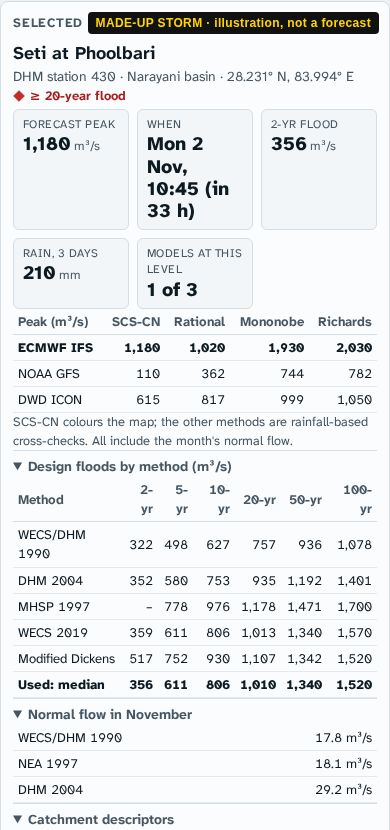
\includegraphics{img/guide/08-point-panel.jpg}

\hypertarget{the-heading}{%
\subsubsection{The heading}\label{the-heading}}

\begin{itemize}
\tightlist
\item
  \textbf{Name}: the river or station name. Smaller streams without a
  name in the river data are called \emph{``Tributary of \ldots{}''}
  (with the named river they join) or \emph{``Unnamed river''}, followed
  by their drainage area.
\item
  \textbf{DHM station number} (for stations), the \textbf{basin}, and
  the coordinates.
\item
  The \textbf{badge} gives the flood level in the chosen view.
\end{itemize}

\hypertarget{the-five-boxes}{%
\subsubsection{The five boxes}\label{the-five-boxes}}

\begin{longtable}[]{@{}lll@{}}
\toprule
\begin{minipage}[b]{0.30\columnwidth}\raggedright
Box\strut
\end{minipage} & \begin{minipage}[b]{0.30\columnwidth}\raggedright
Meaning\strut
\end{minipage} & \begin{minipage}[b]{0.30\columnwidth}\raggedright
In the example\strut
\end{minipage}\tabularnewline
\midrule
\endhead
\begin{minipage}[t]{0.30\columnwidth}\raggedright
\textbf{Forecast peak}\strut
\end{minipage} & \begin{minipage}[t]{0.30\columnwidth}\raggedright
The highest flow forecast \textbf{from now to the end of the forecast},
in m³/s, by the main method (SCS-CN) for the model the view picked\strut
\end{minipage} & \begin{minipage}[t]{0.30\columnwidth}\raggedright
1,180 m³/s\strut
\end{minipage}\tabularnewline
\begin{minipage}[t]{0.30\columnwidth}\raggedright
\textbf{When}\strut
\end{minipage} & \begin{minipage}[t]{0.30\columnwidth}\raggedright
The time of that peak in Nepal time, and how far ahead. \emph{now} means
the flow is highest right now and falling. \emph{No rise forecast} means
it never goes 5\% above its normal flow\strut
\end{minipage} & \begin{minipage}[t]{0.30\columnwidth}\raggedright
Mon 2 Nov, 10:45, in 33 h\strut
\end{minipage}\tabularnewline
\begin{minipage}[t]{0.30\columnwidth}\raggedright
\textbf{2-yr flood}\strut
\end{minipage} & \begin{minipage}[t]{0.30\columnwidth}\raggedright
This point's 2-year flood (median of the formulas). Compare it with the
peak\strut
\end{minipage} & \begin{minipage}[t]{0.30\columnwidth}\raggedright
356 m³/s: the peak is 3.3 times larger\strut
\end{minipage}\tabularnewline
\begin{minipage}[t]{0.30\columnwidth}\raggedright
\textbf{Rain, 3 days}\strut
\end{minipage} & \begin{minipage}[t]{0.30\columnwidth}\raggedright
Mean rain over the catchment in the next 72 hours (the wettest model in
the combined views)\strut
\end{minipage} & \begin{minipage}[t]{0.30\columnwidth}\raggedright
210 mm\strut
\end{minipage}\tabularnewline
\begin{minipage}[t]{0.30\columnwidth}\raggedright
\textbf{Models at this level}, or \textbf{Models ≥ 2-yr}\strut
\end{minipage} & \begin{minipage}[t]{0.30\columnwidth}\raggedright
How many of the three models reach the level of the badge. When the
river is below its 2-year flood, how many reach the 2-year flood at
all\strut
\end{minipage} & \begin{minipage}[t]{0.30\columnwidth}\raggedright
1 of 3: only ECMWF\strut
\end{minipage}\tabularnewline
\bottomrule
\end{longtable}

\hypertarget{peaks-by-model-and-method}{%
\subsubsection{Peaks by model and
method}\label{peaks-by-model-and-method}}

A small table: for each weather model, the forecast peak by each of the
four \textbf{rainfall-based methods}:

\begin{itemize}
\tightlist
\item
  \textbf{SCS-CN} (SCS curve number with the SCS unit hydrograph) is the
  \textbf{main method}. It colours the map and draws the chart. It
  follows the storm hour by hour, takes into account how wet the ground
  is from the last 5 days of rain, and keeps the water of earlier rain
  draining.
\item
  \textbf{Rational}: flow = runoff coefficient × rain intensity over the
  catchment's response time × area. Simple, meant for small catchments
  (up to 50 km²).
\item
  \textbf{Mononobe} and \textbf{Richards}: one peak per day from that
  day's total rain. They are traditional design methods, shown as
  cross-checks.
\end{itemize}

The \textbf{bold row} is the model the current view uses. All values
include the normal flow of the month. When the four methods agree, the
forecast is less sensitive to the choice of formula; when they differ a
lot (as here: 1,180 to 2,030 m³/s for ECMWF), treat the peak as a range,
not one number.

\hypertarget{design-floods-by-method}{%
\subsubsection{Design floods by method}\label{design-floods-by-method}}

The 2- to 100-year floods of each regional formula for this point, and
\textbf{Used: median}, which gives the flood lines on the map and chart.
The \textbf{Chart \textbar{} Table} switch at the top right shows them
as a chart (the default) or as a table; the page remembers your choice
in this browser.

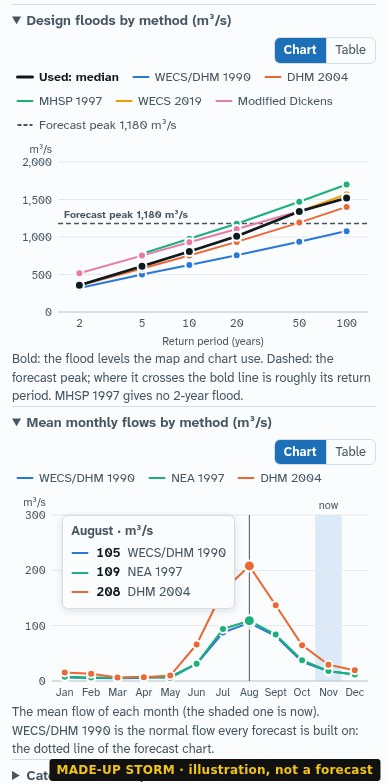
\includegraphics{img/guide/08b-point-charts.jpg}

\begin{itemize}
\tightlist
\item
  \textbf{The chart} has one line per formula: the return period along
  the bottom (2 to 100 years), the flow up the side. The \textbf{bold
  black line} is the median, the flood levels in use. The \textbf{dashed
  line} is the forecast peak: where it crosses the bold line is roughly
  the return period of the forecast flood. Here the peak of 1,180 m³/s
  crosses between the 20-year (1,010) and the 50-year flood (1,340),
  hence the badge \emph{≥ 20-year flood}.
\item
  \textbf{Point at the chart} (tap it on a phone) to read every formula
  at the nearest return period. With a keyboard, Tab to the chart and
  use the arrow keys.
\item
  \textbf{Click a name in the legend} to hide or show its line. The
  scale adjusts to the lines left, which helps when one formula is far
  above the others. \emph{n/a} in the legend means the formula gives no
  value for this point.
\item
  \textbf{The table} has the same numbers. A dash (--) means the formula
  does not give that return period here (MHSP 1997 has no 2-year flood;
  WECS 2019 is not used below 12 km²); on the chart, that line starts
  later or is missing.
\end{itemize}

The spread between the lines shows how uncertain the flood levels
themselves are: for Seti at Phoolbari the 2-year flood is 322 to 517
m³/s depending on the formula.

\hypertarget{mean-monthly-flows-catchment-descriptors-warnings}{%
\subsubsection{Mean monthly flows, catchment descriptors,
warnings}\label{mean-monthly-flows-catchment-descriptors-warnings}}

\begin{itemize}
\tightlist
\item
  \textbf{Mean monthly flows by method}: the mean flow of every month of
  the year by three formulas (WECS/DHM 1990, NEA 1997 and DHM 2004), as
  a chart or a table like the design floods. The shaded month (the bold
  row in the table) is the current one. WECS/DHM 1990 is the base on
  which every forecast is built, the dotted line in the forecast chart.
  The formulas can differ several-fold: DHM 2004 gives about twice as
  much as the other two for catchments with a mean elevation of 1,500 to
  3,000 m, like Seti at Phoolbari (208 against 105 m³/s in August), and
  about a fifth as much in the low Terai.
\end{itemize}

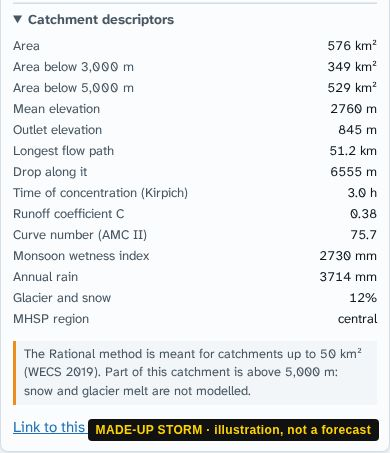
\includegraphics{img/guide/09-point-details.jpg}

\begin{itemize}
\tightlist
\item
  \textbf{Catchment descriptors}: the facts about the catchment that the
  formulas use:
\end{itemize}

\begin{longtable}[]{@{}lll@{}}
\toprule
\begin{minipage}[b]{0.30\columnwidth}\raggedright
Descriptor\strut
\end{minipage} & \begin{minipage}[b]{0.30\columnwidth}\raggedright
What it is\strut
\end{minipage} & \begin{minipage}[b]{0.30\columnwidth}\raggedright
Why it matters\strut
\end{minipage}\tabularnewline
\midrule
\endhead
\begin{minipage}[t]{0.30\columnwidth}\raggedright
Area, area below 3,000 m and 5,000 m\strut
\end{minipage} & \begin{minipage}[t]{0.30\columnwidth}\raggedright
Land draining to this point, in total and below those heights\strut
\end{minipage} & \begin{minipage}[t]{0.30\columnwidth}\raggedright
The flood formulas are based on area: WECS/DHM 1990 and DHM 2004 count
only the land below 3,000 m, Modified Dickens the snow area above 5,000
m\strut
\end{minipage}\tabularnewline
\begin{minipage}[t]{0.30\columnwidth}\raggedright
Mean and outlet elevation\strut
\end{minipage} & \begin{minipage}[t]{0.30\columnwidth}\raggedright
Average height of the catchment, height of the point\strut
\end{minipage} & \begin{minipage}[t]{0.30\columnwidth}\raggedright
Where the water comes from\strut
\end{minipage}\tabularnewline
\begin{minipage}[t]{0.30\columnwidth}\raggedright
Longest flow path, drop along it\strut
\end{minipage} & \begin{minipage}[t]{0.30\columnwidth}\raggedright
Length of the longest route water travels to this point, and how far it
falls\strut
\end{minipage} & \begin{minipage}[t]{0.30\columnwidth}\raggedright
Give the time of concentration\strut
\end{minipage}\tabularnewline
\begin{minipage}[t]{0.30\columnwidth}\raggedright
Time of concentration (Kirpich)\strut
\end{minipage} & \begin{minipage}[t]{0.30\columnwidth}\raggedright
Hours for rain from the farthest part to arrive\strut
\end{minipage} & \begin{minipage}[t]{0.30\columnwidth}\raggedright
Short (≤ 3 h): a flashy river that floods within hours of heavy rain.
Long (a day or more): floods build slowly and last\strut
\end{minipage}\tabularnewline
\begin{minipage}[t]{0.30\columnwidth}\raggedright
Runoff coefficient C, curve number\strut
\end{minipage} & \begin{minipage}[t]{0.30\columnwidth}\raggedright
How much of the rain runs off, from land cover (ESA WorldCover): towns,
ice and fields give higher values than forest\strut
\end{minipage} & \begin{minipage}[t]{0.30\columnwidth}\raggedright
Higher = more flood per mm of rain\strut
\end{minipage}\tabularnewline
\begin{minipage}[t]{0.30\columnwidth}\raggedright
Monsoon wetness index, annual rain\strut
\end{minipage} & \begin{minipage}[t]{0.30\columnwidth}\raggedright
Mean June-September and annual rain over the catchment (ERA5
2019-2023)\strut
\end{minipage} & \begin{minipage}[t]{0.30\columnwidth}\raggedright
Used by the normal-flow formulas; too wet over the hills
(\protect\hyperlink{13-what-the-forecast-cannot-tell-you}{section
13})\strut
\end{minipage}\tabularnewline
\begin{minipage}[t]{0.30\columnwidth}\raggedright
Glacier and snow\strut
\end{minipage} & \begin{minipage}[t]{0.30\columnwidth}\raggedright
Share of the catchment under ice and snow\strut
\end{minipage} & \begin{minipage}[t]{0.30\columnwidth}\raggedright
Melt is not modelled\strut
\end{minipage}\tabularnewline
\begin{minipage}[t]{0.30\columnwidth}\raggedright
MHSP region\strut
\end{minipage} & \begin{minipage}[t]{0.30\columnwidth}\raggedright
Western, central or eastern Nepal\strut
\end{minipage} & \begin{minipage}[t]{0.30\columnwidth}\raggedright
Chooses the MHSP 1997 coefficients\strut
\end{minipage}\tabularnewline
\bottomrule
\end{longtable}

\begin{itemize}
\tightlist
\item
  \textbf{Warnings} (orange box) appear when a method is outside its
  range: the Rational method above 50 km², a catchment partly above
  5,000 m (snow and glacier melt are missing), a time of concentration
  over 24 h (daily methods do not apply), or a very large river (over
  5,000 km², whose floods come from far upstream over days).
\item
  \textbf{Link to this point}: a web address that opens the page on this
  river; see
  \protect\hyperlink{12-on-a-phone-and-sharing-a-river}{section 12}.
\end{itemize}

\hypertarget{how-many-numbers-become-one-colour}{%
\subsection{9. How many numbers become one
colour}\label{how-many-numbers-become-one-colour}}

Behind every river there are 3 weather models × 4 rainfall methods × 6
return periods × 5 flood formulas. The page reduces them in fixed steps:

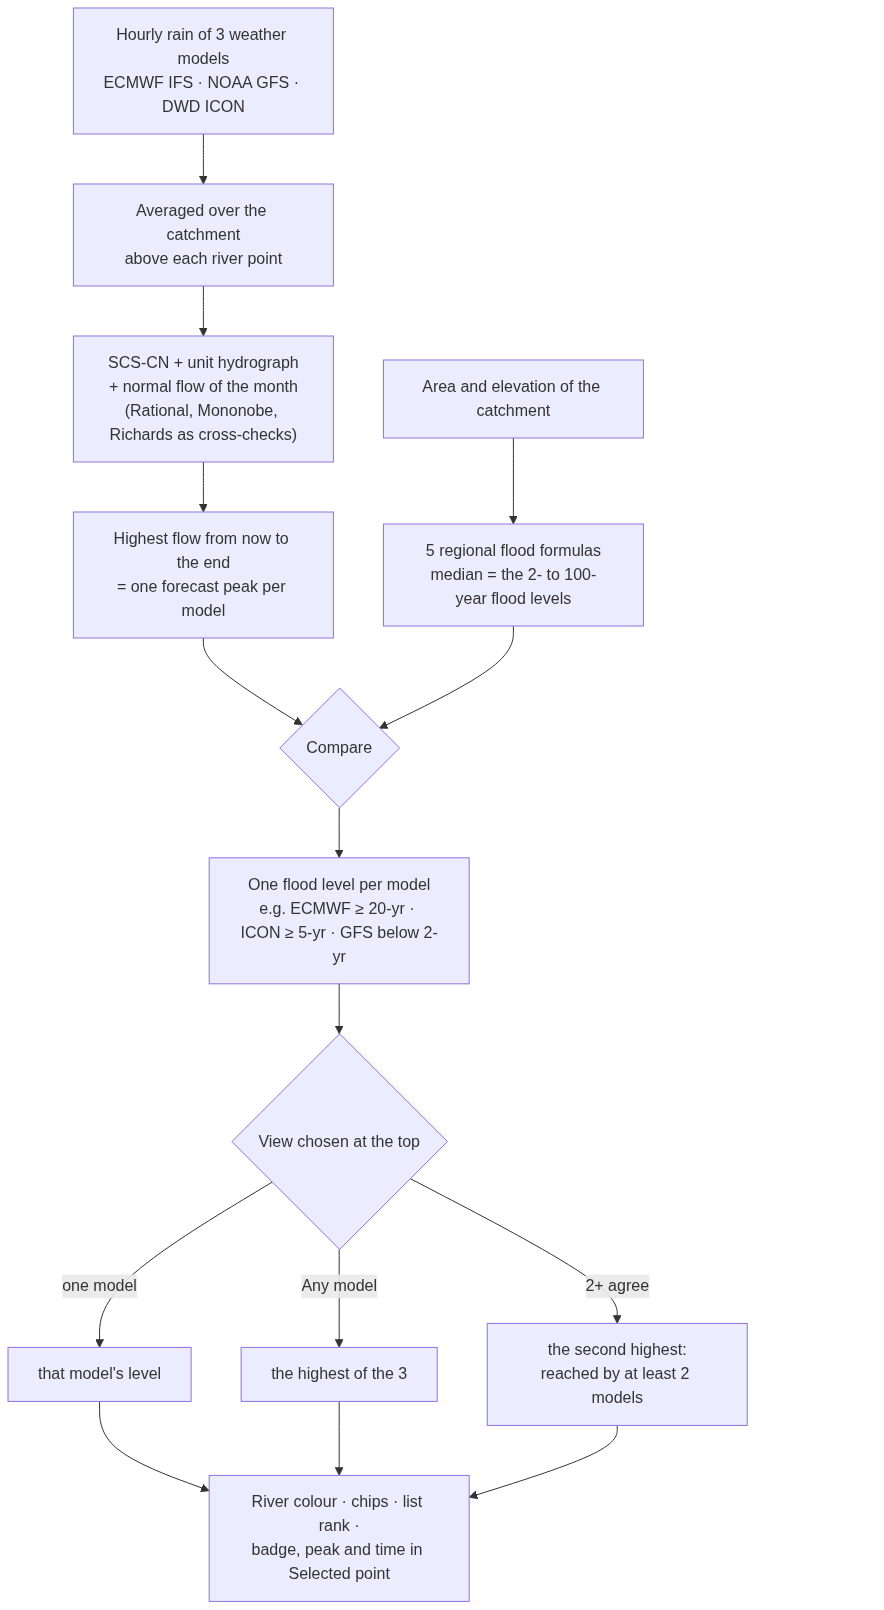
\includegraphics[width=0.7\textwidth,height=\textheight]{img/guide/09-diagram.png}

\textbf{Worked example}: Seti at Phoolbari in the made-up storm. Its
flood levels (median row) are 356 (2-yr), 611 (5-yr), 806 (10-yr), 1,010
(20-yr), 1,340 (50-yr) and 1,520 m³/s (100-yr). The three models give
these SCS-CN peaks:

\begin{longtable}[]{@{}lll@{}}
\toprule
Model & Peak & Highest level reached\tabularnewline
\midrule
\endhead
ECMWF IFS & 1,180 m³/s & ≥ 20-year (above 1,010, below
1,340)\tabularnewline
DWD ICON & 615 m³/s & ≥ 5-year (just above 611)\tabularnewline
NOAA GFS & 110 m³/s & below the 2-year flood\tabularnewline
\bottomrule
\end{longtable}

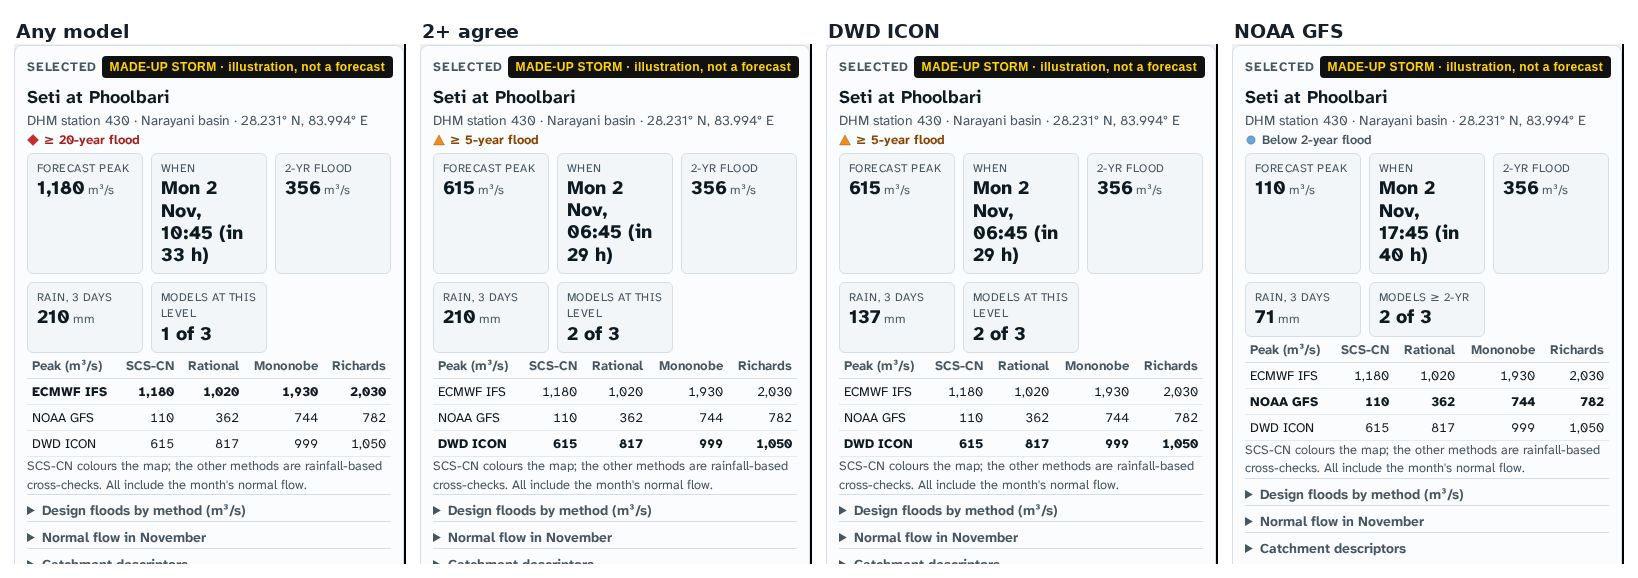
\includegraphics{img/guide/10-point-in-four-views.jpg}

\begin{itemize}
\tightlist
\item
  \textbf{Any model} takes the highest, ECMWF: ◆ \emph{≥ 20-year flood},
  peak 1,180 m³/s on Monday 10:45, \textbf{1 of 3} models at this level.
\item
  \textbf{2+ agree} takes the second highest, ICON: ▲ \emph{≥ 5-year
  flood}, peak 615 m³/s on Monday 06:45, \textbf{2 of 3} models (ECMWF
  and ICON both reach at least the 5-year flood).
\item
  \textbf{DWD ICON} alone gives the same level and peak, but its own
  3-day rain (137 mm instead of the wettest model's 210 mm).
\item
  \textbf{NOAA GFS} alone: \emph{below 2-year flood}, peak 110 m³/s. The
  box reads \emph{Models ≥ 2-yr: 2 of 3}, a reminder that the other two
  models do flood this river.
\end{itemize}

How to read it: \emph{``A flood is likely here on Monday morning. Two
models say at least a 5-year flood, one says a 20-year flood, one sees
almost nothing. Watch the next updates.''} When two models agree on the
level of a flood, the forecast is stronger than when only one model
shows it.

When two models reach the same level, the view takes the one with the
larger rise. The bold row of the peaks table always shows which model
the view is using.

\hypertarget{the-forecast-chart-hydrograph}{%
\subsection{10. The forecast chart
(hydrograph)}\label{the-forecast-chart-hydrograph}}

\emph{Made-up storm, Any model, mouse over the ECMWF peak.}

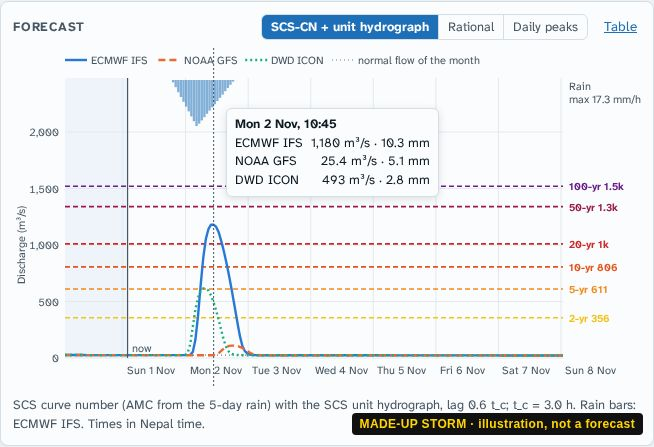
\includegraphics{img/guide/11-chart-scs.jpg}

\begin{longtable}[]{@{}ll@{}}
\toprule
\begin{minipage}[b]{0.47\columnwidth}\raggedright
Element\strut
\end{minipage} & \begin{minipage}[b]{0.47\columnwidth}\raggedright
Meaning\strut
\end{minipage}\tabularnewline
\midrule
\endhead
\begin{minipage}[t]{0.47\columnwidth}\raggedright
Horizontal axis\strut
\end{minipage} & \begin{minipage}[t]{0.47\columnwidth}\raggedright
Time in Nepal time, from 24 hours ago (shaded) to the end of the
forecast\strut
\end{minipage}\tabularnewline
\begin{minipage}[t]{0.47\columnwidth}\raggedright
\textbf{now} line\strut
\end{minipage} & \begin{minipage}[t]{0.47\columnwidth}\raggedright
The present. Left of it: what the models' rain did; right: the
forecast\strut
\end{minipage}\tabularnewline
\begin{minipage}[t]{0.47\columnwidth}\raggedright
Coloured lines\strut
\end{minipage} & \begin{minipage}[t]{0.47\columnwidth}\raggedright
Flow by model: ECMWF solid blue, GFS dashed orange, ICON dotted
green\strut
\end{minipage}\tabularnewline
\begin{minipage}[t]{0.47\columnwidth}\raggedright
Dotted grey line\strut
\end{minipage} & \begin{minipage}[t]{0.47\columnwidth}\raggedright
The normal flow of the month, the base under every forecast\strut
\end{minipage}\tabularnewline
\begin{minipage}[t]{0.47\columnwidth}\raggedright
Blue bars hanging from the top\strut
\end{minipage} & \begin{minipage}[t]{0.47\columnwidth}\raggedright
Hourly catchment rain (of ECMWF in the combined views, of the chosen
model otherwise); the largest hourly amount is written at the right
(``max 17.3 mm/h'')\strut
\end{minipage}\tabularnewline
\begin{minipage}[t]{0.47\columnwidth}\raggedright
Dashed horizontal lines\strut
\end{minipage} & \begin{minipage}[t]{0.47\columnwidth}\raggedright
The flood levels: 2-yr yellow up to 100-yr purple, labelled at the
right\strut
\end{minipage}\tabularnewline
\begin{minipage}[t]{0.47\columnwidth}\raggedright
``Above the chart: \ldots{}''\strut
\end{minipage} & \begin{minipage}[t]{0.47\columnwidth}\raggedright
Flood levels too high to fit: the forecast stays well below them\strut
\end{minipage}\tabularnewline
\begin{minipage}[t]{0.47\columnwidth}\raggedright
Mouse over\strut
\end{minipage} & \begin{minipage}[t]{0.47\columnwidth}\raggedright
A vertical line and a box with the time, each model's flow and its rain
in that hour\strut
\end{minipage}\tabularnewline
\bottomrule
\end{longtable}

What to read from it:

\begin{itemize}
\tightlist
\item
  \textbf{Which flood lines a model line crosses}, and \textbf{for how
  long}.
\item
  \textbf{Timing.} The gap between the rain bars and the peak is the
  catchment's response time: about 6 hours for this 576 km² river (time
  of concentration 3 h). Big rivers respond over a day or more.
\item
  \textbf{Agreement.} Here ECMWF rises to 1,180 m³/s, ICON peaks earlier
  at 615 and GFS hardly moves: the models disagree on how much rain
  falls \emph{on this catchment}.
\item
  \textbf{Rising or falling.} If the highest point is at the \emph{now}
  line, the river is past its peak.
\end{itemize}

The buttons above the chart switch the method, and \textbf{Table} lists
the numbers:

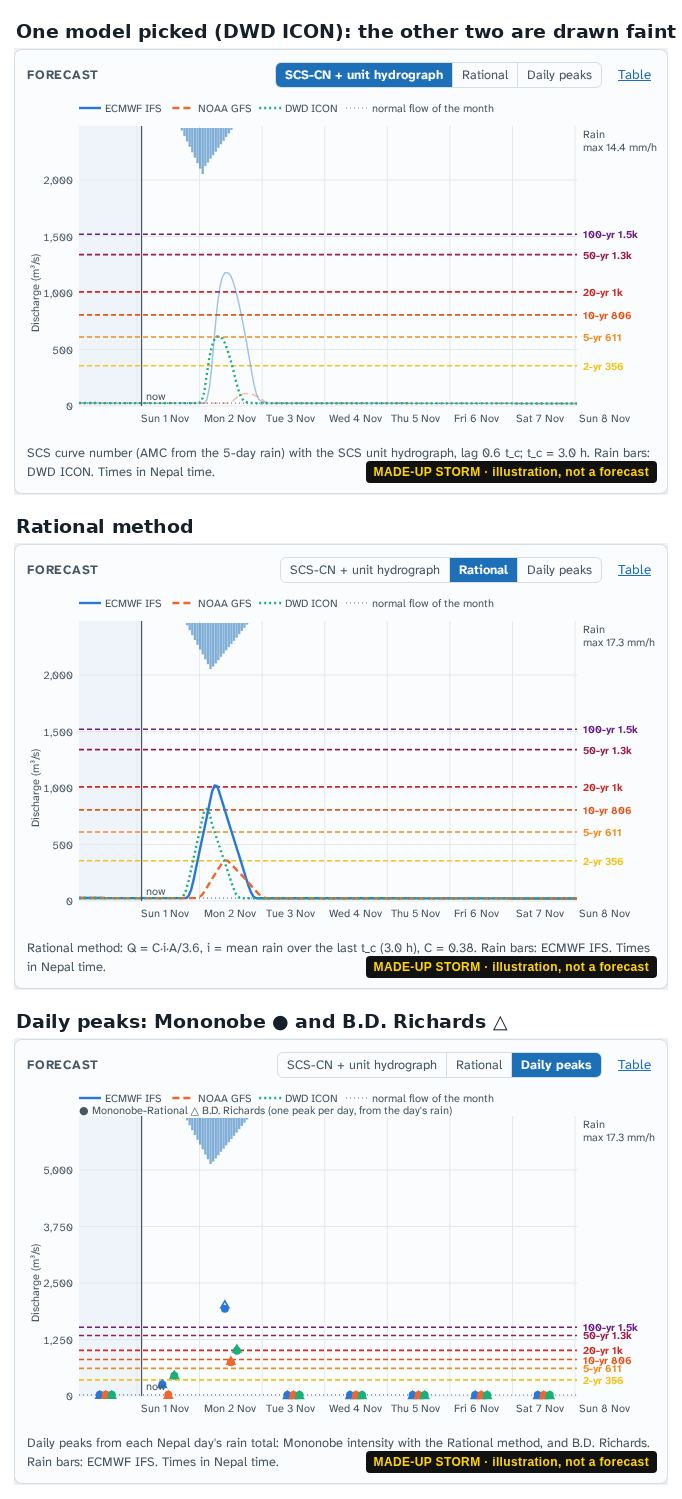
\includegraphics{img/guide/12-chart-methods.jpg}

\begin{itemize}
\tightlist
\item
  \textbf{Picking one model} at the top draws its line bold and the
  other two faint, and shows its own rain bars.
\item
  \textbf{Rational} responds to rain at once and drops as soon as it
  stops: a cross-check, meant for small catchments.
\item
  \textbf{Daily peaks} shows one point per day and model: ●
  Mononobe-Rational and △ B.D. Richards, computed from each day's rain
  total.
\item
  \textbf{Table} gives the values every 3 hours: flow and rain (over
  those 3 hours) for each model, and the normal flow, for copying into a
  report or a spreadsheet.
\end{itemize}

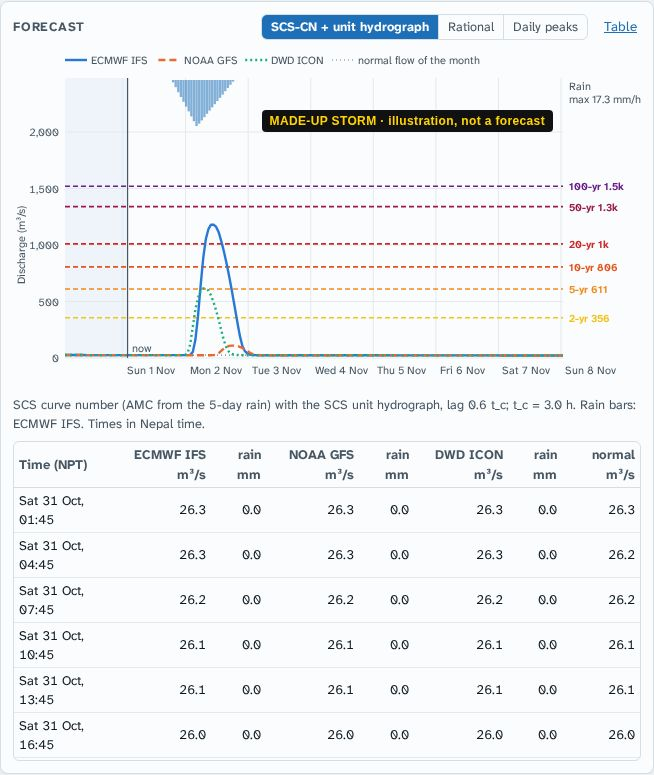
\includegraphics{img/guide/13-chart-table.jpg}

\hypertarget{reading-a-quiet-day}{%
\subsection{11. Reading a quiet day}\label{reading-a-quiet-day}}

\emph{Real, 1 November 2026: Sunkoshi at Pachuwarghat (DHM station
630).}

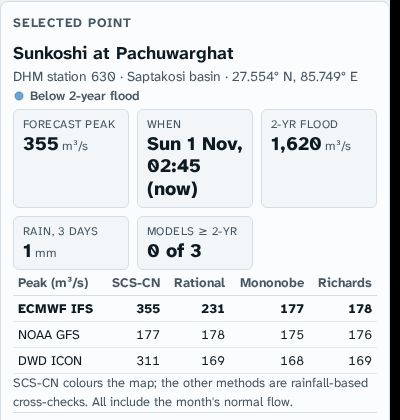
\includegraphics{img/guide/14-real-quiet-kpis.jpg}
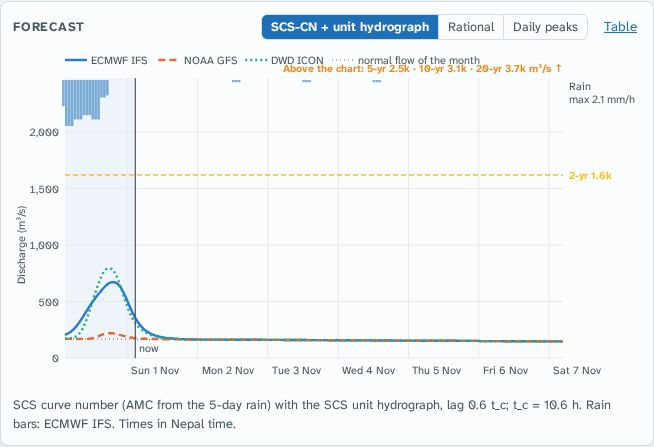
\includegraphics{img/guide/14-real-quiet-chart.jpg}

\begin{itemize}
\tightlist
\item
  \textbf{When: \ldots{} (now).} The highest flow of the forecast is
  right now. The chart shows why: a little rain fell in the last day
  (the bars in the shaded past), the river rose, and from now on it
  falls back towards its normal flow.
\item
  \textbf{Forecast peak 355 m³/s vs 2-yr flood 1,620 m³/s}: about a
  fifth of the 2-year flood. \emph{Models ≥ 2-yr: 0 of 3}, \emph{Rain, 3
  days: 1 mm}. Nothing to watch.
\item
  The chart shows only the 2-year line; the higher ones are listed as
  \emph{``Above the chart''}.
\item
  In the peaks table the daily methods (Mononobe 177, Richards 178) are
  lower than SCS-CN (355): they only see each future day's rain, which
  is almost zero, while SCS-CN still carries the water of the past rain
  draining out.
\item
  In the Hotspots list the same river reads \emph{``rises 13\% of the
  way to its 2-yr flood · peak 355 m³/s now''}. \emph{Rises} is measured
  from the normal flow of the month, not from the present flow: the
  river is 13\% of the way from normal to its 2-year flood, and falling.
\end{itemize}

\hypertarget{on-a-phone-and-sharing-a-river}{%
\subsection{12. On a phone, and sharing a
river}\label{on-a-phone-and-sharing-a-river}}

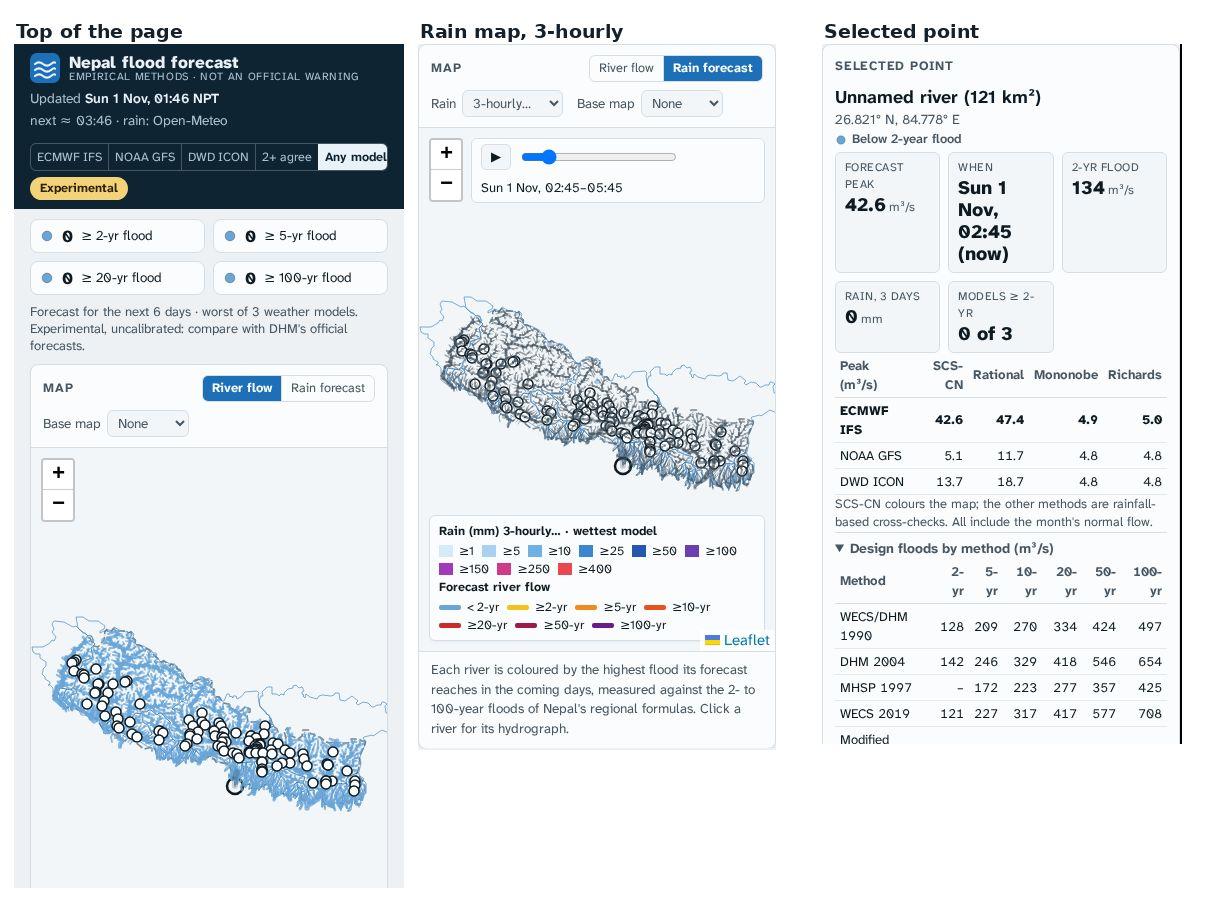
\includegraphics{img/guide/15-phone.jpg}

On a narrow screen the parts are stacked: the summary and map first,
then the chart, the selected point and the list. Everything works the
same; the view buttons scroll sideways if they do not fit.

\textbf{Sharing.} Click \textbf{Link to this point}, or simply copy the
address from the browser after selecting a river: it ends in
\texttt{\#t=2048\&m=any} (point number and view). Whoever opens it gets
the same river in the same view, with the newest forecast.

\hypertarget{what-the-forecast-cannot-tell-you}{%
\subsection{13. What the forecast cannot tell
you}\label{what-the-forecast-cannot-tell-you}}

\begin{itemize}
\tightlist
\item
  \textbf{It is not calibrated.} The formulas have not been tuned
  against floods measured at these rivers. Use the levels to compare
  rivers and days, not as exact predictions.
\item
  \textbf{Rain only.} Snow and glacier melt, glacial lake outbursts
  (GLOFs), landslide dams, dam releases and embankment breaches are not
  in it.
\item
  \textbf{Weather-model rain is coarse} (9 to 25 km). It misses small,
  intense thunderstorms, which cause flash floods in the Chure and small
  hill streams. A blue small river is not a promise that it will stay
  calm.
\item
  \textbf{Big Himalayan rivers} (Koshi, Narayani, Karnali) get their
  floods from far upstream over days, partly from snowmelt; the
  empirical methods are rough there.
\item
  \textbf{The normal flow runs high in the hills} (the climate data used
  is too wet there), so the base under the forecast is generous in the
  hills.
\item
  \textbf{The forecast is only as good as the last update.} Check the
  update time, and expect rain forecasts beyond 3 days to change.
\end{itemize}

\hypertarget{questions-people-ask}{%
\subsection{14. Questions people ask}\label{questions-people-ask}}

\textbf{Every river is blue. Is the page working?} Yes, if the update
time is recent. In the dry season most days are like this. The Hotspots
list still shows the rivers rising the most.

\textbf{Why does a river show a flood in ``Any model'' but not in ``2+
agree''?} Only one model brings enough rain to that catchment. Look at
that river's chart: if the other two models also rise but stay just
below the line, the signal is stronger than if they stay flat.

\textbf{Why do the models disagree so much?} Heavy rain in the mountains
is hard to forecast; a shift of 30 km moves the rain into another
valley. Disagreement is information: it tells you the forecast is
uncertain.

\textbf{The peak says ``now'' but no rain is forecast. Why is the flow
above normal?} Water from rain that has already fallen is still
draining. The flow is falling back to normal.

\textbf{Why is the forecast peak at a station different from what DHM
measures?} The page estimates flows with formulas from rain forecasts;
DHM measures water levels. Differences of a factor of two are possible.
Trust the measurements and DHM's official forecast.

\textbf{How far ahead can I trust it?} The first 1 to 2 days are the
most reliable. Beyond 3 days, treat a flood signal as an early heads-up
and watch whether it persists through the next updates.

\textbf{Why do some rivers have no name?} Names come from the DHM
station list: a river is named along its main stem wherever a DHM
station names it. Other streams are named after the named river they
join (``Tributary of \ldots{}''), or called ``Unnamed river'' with their
drainage area.

\hypertarget{glossary}{%
\subsection{15. Glossary}\label{glossary}}

\begin{longtable}[]{@{}ll@{}}
\toprule
\begin{minipage}[b]{0.47\columnwidth}\raggedright
Term\strut
\end{minipage} & \begin{minipage}[b]{0.47\columnwidth}\raggedright
Meaning\strut
\end{minipage}\tabularnewline
\midrule
\endhead
\begin{minipage}[t]{0.47\columnwidth}\raggedright
\textbf{m³/s}\strut
\end{minipage} & \begin{minipage}[t]{0.47\columnwidth}\raggedright
Cubic metres per second: the flow of a river. 1 m³/s is 1,000 litres
every second\strut
\end{minipage}\tabularnewline
\begin{minipage}[t]{0.47\columnwidth}\raggedright
\textbf{Discharge, flow}\strut
\end{minipage} & \begin{minipage}[t]{0.47\columnwidth}\raggedright
How much water passes a point of the river per second\strut
\end{minipage}\tabularnewline
\begin{minipage}[t]{0.47\columnwidth}\raggedright
\textbf{Catchment, drainage area}\strut
\end{minipage} & \begin{minipage}[t]{0.47\columnwidth}\raggedright
All the land whose rain drains to a point of the river, in km²\strut
\end{minipage}\tabularnewline
\begin{minipage}[t]{0.47\columnwidth}\raggedright
\textbf{Return period, T-year flood}\strut
\end{minipage} & \begin{minipage}[t]{0.47\columnwidth}\raggedright
A flow reached or exceeded on average once every T years (a 1/T chance
in any year)\strut
\end{minipage}\tabularnewline
\begin{minipage}[t]{0.47\columnwidth}\raggedright
\textbf{Flood level}\strut
\end{minipage} & \begin{minipage}[t]{0.47\columnwidth}\raggedright
Here: the 2- to 100-year floods of a point, the median of five regional
formulas\strut
\end{minipage}\tabularnewline
\begin{minipage}[t]{0.47\columnwidth}\raggedright
\textbf{Normal flow}\strut
\end{minipage} & \begin{minipage}[t]{0.47\columnwidth}\raggedright
The mean flow of the month, from regional formulas\strut
\end{minipage}\tabularnewline
\begin{minipage}[t]{0.47\columnwidth}\raggedright
\textbf{Hydrograph}\strut
\end{minipage} & \begin{minipage}[t]{0.47\columnwidth}\raggedright
A chart of flow against time\strut
\end{minipage}\tabularnewline
\begin{minipage}[t]{0.47\columnwidth}\raggedright
\textbf{Time of concentration (t\_c)}\strut
\end{minipage} & \begin{minipage}[t]{0.47\columnwidth}\raggedright
The time for rain from the farthest part of the catchment to reach the
point\strut
\end{minipage}\tabularnewline
\begin{minipage}[t]{0.47\columnwidth}\raggedright
\textbf{SCS-CN}\strut
\end{minipage} & \begin{minipage}[t]{0.47\columnwidth}\raggedright
The US Soil Conservation Service curve-number method: how much rain runs
off, depending on land cover and how wet the ground is\strut
\end{minipage}\tabularnewline
\begin{minipage}[t]{0.47\columnwidth}\raggedright
\textbf{Unit hydrograph}\strut
\end{minipage} & \begin{minipage}[t]{0.47\columnwidth}\raggedright
How a catchment spreads a burst of runoff out in time\strut
\end{minipage}\tabularnewline
\begin{minipage}[t]{0.47\columnwidth}\raggedright
\textbf{Reach}\strut
\end{minipage} & \begin{minipage}[t]{0.47\columnwidth}\raggedright
A stretch of river between two junctions; the page forecasts each reach
at its downstream end\strut
\end{minipage}\tabularnewline
\begin{minipage}[t]{0.47\columnwidth}\raggedright
\textbf{NPT}\strut
\end{minipage} & \begin{minipage}[t]{0.47\columnwidth}\raggedright
Nepal time, UTC + 5:45. All times on the page are Nepal time\strut
\end{minipage}\tabularnewline
\begin{minipage}[t]{0.47\columnwidth}\raggedright
\textbf{ECMWF, GFS, ICON}\strut
\end{minipage} & \begin{minipage}[t]{0.47\columnwidth}\raggedright
The European, US and German global weather models\strut
\end{minipage}\tabularnewline
\begin{minipage}[t]{0.47\columnwidth}\raggedright
\textbf{DHM}\strut
\end{minipage} & \begin{minipage}[t]{0.47\columnwidth}\raggedright
The Department of Hydrology and Meteorology of Nepal, the official
source of flood forecasts and warnings\strut
\end{minipage}\tabularnewline
\bottomrule
\end{longtable}

\begin{center}\rule{0.5\linewidth}{0.5pt}\end{center}

\emph{Screenshots: the real ones are the forecast of 1 November 2026,
01:46 NPT. The made-up storm puts up to 260 mm of rain in a day on
central Nepal, differently for each model, and was run through the same
code locally. It was never published as a forecast.}

\end{document}
